%! Author = jaroslav
%! Date = 20.03.20
\chapter{ЛИТЕРАТУРНЫЙ ОБЗОР}
\section{Определение основных понятий}

Под \glqqрешениями\grqq{ } будем~понимать совокупность рассматриваемых возможностей, которые выделены тем
или иным способом человеком, группой лиц или внешней средой.~Этой терминологии в иностранном языке
соответствует слово "decision".
Тогда, принятие решения - это процесс выбора определенной возможности человеком или группой лиц.
Проблемой принятия решения занимаются многие дисциплины: теория принятия решений, системный анализ,
теория статистических~решений, информатика, искусственный интеллект, когнитивная психология, теория
поведения, теория игр и др.
Теория принятия решений в основном занимается разработкой различных методов и средств, необходимых
человеку для формулировки вариантов решения проблемы, нахождением наилучшего решения проблемы и
обоснованием выбора решения~\citep{petrovsky2009theory}.
В применение к когнитивной психологии, теория принятия решений используется для изучения причин выбора
определенного решения человеком.
Имеются задачи, которые могут иметь комплекс различных дисциплин, например включать в себя теорию игр,
когнитивную психологию и исскуственный интеллект.
Такие задачи обычно относят к теории принятия решений и не рассматривают отдельно друг от друга.
Примером тому является эксперимент одноразовой дилеммы заключенного, о котором будет рассказано далее.

В теории принятия решений существует большое количество классификаций проблем, связанных с различным
сферами развития в других науках, одним из которых является понятия риск и неопределенность.
В широком смысле, "неопределенность" трактуется неоднозначно и зависит от условий решаемой задачи.
Для описания неопределенности, теория принятия решения применяет, в частности, инструмент теории
нечетких множетв~\citep{demidiva2012decision}. Теория нечетких множеств позволяет отнести некоторое
множество $X$ к некоторому подмножеству $A$, используя параметр степени принадлежности $\mu_{A}$.
Степень принадлежности является функцией и принимает зачения в интервале $[0,1]$.
В формальном виде, нечеткое множество можно описать следующим образом: $A = \{(x,\mu_{A}(x)) | x \in X\}$.

Помимо инструментов для описания неопределенности большинства наук, в когнитивной психологии, существует большое
количество концепций, по которым описывается поведение человека. Одним из таких концепций
является прицип уверенности Сэвиджа. Этот принцип гласит, если положительный результат события $S$
дает выбор решения $R$, отрицательный результат события $\bar{S}$ дает выбор решения $R$, тогда
отсутсвие информации о событии $S$ даст выбор решения $R$. Иначе говоря, событие $S$ никак
не влияет на выбор решения, даже если событие $S$ неопределено. В таком понимании, неопределенность
понимается как неоднозначность объективного состояния мира. Принцип уверенности Сэвиджа показывает
рациональное мышление. Однако, принцип Сэвиджа нарушается в ряде экспериментов, где тому пример
эксперимент с эффектом неоднозначности Эллсберга~\citep{daniel1961risk} и эксперимент с покупкой
билета~\citep{tversky1992disjunction}.

%%%%%%%%%%%%%%%%%%%%%%%%%%%%%%%%%%%%%%%%%%%%%%%%%%%%%%%%%%%%%%%%%%%%%%%%%%%%%%%%%%%%%%%%%%%%%%%%%%%%
%%%%%%%%%%%%%%%%%%%%%%%%%%%%%%%%%%%%%%%%%%%%%%%%%%%%%%%%%%%%%%%%%%%%%%%%%%%%%%%%%%%%%%%%%%%%%%%%%%%%
\section{Эксперимент Эллсберга. Дилемма студента}

Первым примером рассмотрим эффект неоднозначности Эллсберга. Данный эффект формулирутеся
в мысленном эксперименте, когда имеются две урны, в каждой из которых по 100 мячей, где в первой
урне 50 красных и 50 черных, во второй соотношение неизвестно. Участникам эксперимента задается
вопрос: "Какую выберете урну, чтобы достать черный мяч?". В случае угадывания испытуемый получает денежное
вознаграждение, иначе ничего не теряет~\citep{daniel1961risk}. Для данной задачи был проведен эксперимент,
большинство испытуемых были склонны выбирать первую урну, иначе говоря большинство человек решило рискнуть,
поскольку вероятность вынуть черный мяч 50/50. А неопределенность второй урны было не привлекательным,
хотя соотношение внутри этой урны могло быть 70/30, 90/10 или даже 100/0, хотя при проигрыше игрок ничего
не терял~\citep{daniel1961risk}~\citep{dominiak2012dynamic}~\citep{camerer1992recent}. Иллюстрация
этого эксперимента приведена на рисунке~\ref{fig:expmnt_ellsberg}

\begin{figure}[h!]
    \centering
    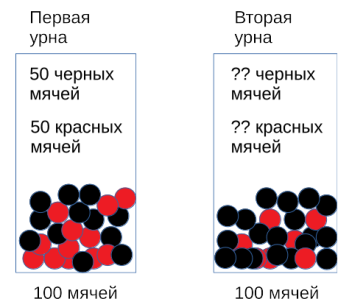
\includegraphics[width=0.5\linewidth]{pictures/pic_expmnt_ellsberg.png}
    \caption{Эксперимент Эллсберга характеризующее когнитивное искажение, в котором принятие решения
    страдает из-за недостатка информации. В эксперименте предпочтительней будет первая урна, для
    которой вероятность благоприятного исхода известна, нежели вторая, где вероятность
    благоприятного исхода неизвестна.}
    \label{fig:expmnt_ellsberg}
\end{figure}

Более простым примером неопределенности является ситуация связанности независимых событий. Например,
студент плохо готов к экзамену, поэтому ему надо решить, либо идти на экзамен и попытаться
защититься, либо пропустить экзамен и пойти на дополнительную попытку. При этом, студент хочет
полететь на отдых, для чего необходимо купить билеты заранее. Эти два вопроса, о экзамене и покупке
билетов, никак не связаны, однако, студент может быть не удовлетворен результатом экзамена и не полететь
или не сдавать экзамен и спокойно полететь. Иллюстрация этих возможных вариантов событий представлена
на рисунке~\ref{fig:vac_exam}

%\begin{figure}
%    \begin{minipage}[h]{0.4\linewidth}
%        \center{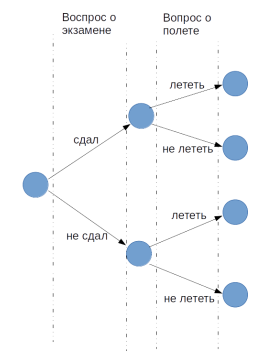
\includegraphics[width=1\linewidth]{pictures/vacation_and_exam.png} \\ а)}
%    \end{minipage}
%    \hfill
%    \begin{minipage}[h]{0.4\linewidth}
%        \center{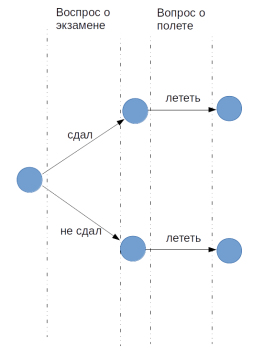
\includegraphics[width=1\linewidth]{pictures/vacation_and_exam_2.png} \\ б)}
%    \end{minipage}
%    \caption{Цепочка событий для двух вопросов a)из эксперимента \citep{shafir199228thinking}, б)по принципу Сэвиджа}
%\end{figure}

\newpage
\begin{figure}[h!]
    \centering
    \captionsetup{justification=centering}
    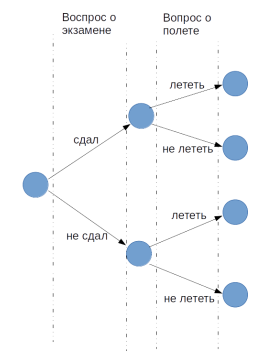
\includegraphics[width=0.35\linewidth]{pictures/vacation_and_exam.png}
    \caption{Цепь возможных исходов независимых событий~\citep{shafir199228thinking}}
    \label{fig:vac_exam}
\end{figure}
где кругами обозначаются определенные состояния события. Если использовать принцип уверенности Сэвиджа,
то варианты событий будут выглядеть как на рисунке~\ref{fig:vac_exam_savage}

\begin{figure}[h!]
    \centering
    \captionsetup{justification=centering}
    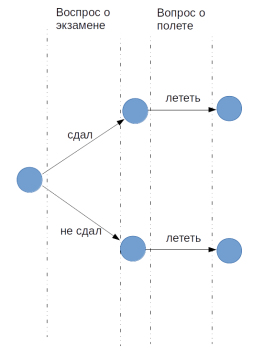
\includegraphics[width=0.35\linewidth]{pictures/vacation_and_exam_2.png}
    \caption{Цепь возможных исходов, образованных по принципу Сэвиджа}
    \label{fig:vac_exam_savage}
\end{figure}
Из этого рисунка видно, что человек всегда выберет один вариант для второго вопроса и при этом ответ
на первый вопрос никак не влияет на второй вопрос. Однако, в этом эксперименте было получено, что
многие люди решили купить билеты в случае провала экзамена или в случае сдачи, но решили не покупать
в случае неизвестных результатов экзамена~\citep{tversky1992disjunction}.

Важным результатом этих экспериментов является выявление эффекта дизъюнкции. Эффект дизъюнкции гласит,
что лучше выбрать вариант $x$ чем $y$, если известно о результате события $S$, или лучше выбрать
вариант $y$ чем $x$, если о результате события $S$ ничего не известно. Данный эффект был сформулирован
в работе Шафира и Тверского~\citep{shafir199228thinking}.

%%%%%%%%%%%%%%%%%%%%%%%%%%%%%%%%%%%%%%%%%%%%%%%%%%%%%%%%%%%%%%%%%%%%%%%%%%%%%%%%%%%%%%%%%%%%%%%%%%%%
%%%%%%%%%%%%%%%%%%%%%%%%%%%%%%%%%%%%%%%%%%%%%%%%%%%%%%%%%%%%%%%%%%%%%%%%%%%%%%%%%%%%%%%%%%%%%%%%%%%%
\section{Роль когнитивных искажений в принятии решений}

Еще один пример с связан ошибкой конъюнкции, который был получен в эксперименте Тверского и
Канемана~\citep{tversky1983extensional}. Эксперимент показывает, что для человека некоторые составные
факты могут быть весомее общих. Для постановки эксперимента, каждому участнику дается информация о
Линде. "Ей 31 год, она одинокая, искренная и очень яркая. Она училась на факультете философии.
Будучи студенткой была обеспокоена вопросами дискриминации и социальной несправедливости, участвовала
в демонстрациях против ядерного оружия". После задавался вопрос: "Какой факт о Линде более вероятен?"
\begin{itemize}
    \item "Линда - кассир в банке";
    \item "Линда - кассир в банке и активная феминистка";
\end{itemize}
Для эксперимента были отобраны 142 студента магистратуры. Для одной половины студентов порядок альтернатив
был прямой, для других обратный, но эта манипуляция не принесла других результатов. В результате 85\%
респондентов выбрали второй вариант: "Линда - кассир в банке и активная феминистка"\citep{tversky2004extensional}.

Эти эффекты показывают, что люди не оценивают все ветви соответствующего дерева решений, даже если
количество результатов велико.

Помимо принятия решения~человеком в условиях неопределенности событий, в когнитивной психологии~рассматриваются
задачи в условиях неопределенности результата решения других людей. Ярким примером такой неопределенности
является дилемма~заключенного. Разница между предыдущими экспериментами заключается в раскрытии большей
информации о неопределенности. Другими словами, респонденту будет известна предположительная информация
о выборе другого человека. Таким образом, предполагается раскрыть больше информации об когнитивных эффектах
происходящих в условиях неопределенности.

Дилемма заключенного является основной задачей теории игр и уже имеет большое количество направлений
исследования. Самым интересным направлением стоит отметить исследования повторяющихся игр, тоесть когда
дилемма заключенного повторяется по неколько раз с теми же игроками. Но не менее интересным стоит
отметить игры на один раз в контексте когнитивной психологии. Разница между многократной и одиночной
игрой заключается в степени неопределенности. Человек абсолютно не знает о другом человеке в первую игру и
не может определить тактику другого человека. При многократном повторении игроки могут угадывать
поведение другого и таким образом неопределеность начинает исчезать.

Но что будет, если игрок будет знать о другом предположительную информацию. В этом случае результат для
первых экспериментов был неожиданным, в них наблюдались эффект неоднозначности и эффект дизъюнкции.
Для объяснения всей сути проблемы необходимо начать с постановки задачи.

В игре учавствуют двое заключенных, каждого из которых поймали во время преступления. Каждому заключенному
дается выбор либо предать друого, либо молчать. Их общий выбор будет влиять на величину наказания для
обоих согласно таблице~\ref{tabular:table_pay}:

\newpage
\begin{table}[h!]
    \caption{Таблица выплат для классической задачи}
    \label{tabular:table_pay}
    \begin{tabular}{cccc}
        "" & "" & \multicolumn{2}{c}{заключенный Б} \\
        "" & "" & молчать & предать \\
        заключенный А &
        \begin{tabular}{r}
            молчать \\
            "" \\
            предать \\
        \end{tabular} &
        \begin{tabular}{|c|}
            \hline
            А - 0.5 года \\
            Б - 0.5 года\\
            \hline
            А - свободен \\
            Б - 10 лет \\
            \hline
        \end{tabular} &
        \begin{tabular}{|c|}
            \hline
            А - 10 лет \\
            Б - свободен \\
            \hline
            А - 2 года \\
            Б - 2 года \\
            \hline
        \end{tabular}
    \end{tabular}
\end{table}
Каждый заключенный знает про эту таблицу и пытается свести результат к минимальному возможному наказанию.
Согласно теории игр, каждому заключенному по Парето-оптимуму необходимо выбирать вариант молчать.
Парето-оптимум позволяет рассматривать задачу для обоих заключенных, позволяет найти общий выйгрыш
для двух заключенных. Рассмотрение задачи для каждого в отдельности позволяет прийти к выводу, что
самым лучшим вариантом является предательство. Поскольку в случае предательства одного заключенного,
промолчавший заключенный получает максимальное наказание. Случай с предательством обоими заключеными
является равновесием Нэша. Согласно равновесию Нэша, существует стратегия или набор стратегий,
изменив которые невозможно получить больший выйгрыш, если друие игроки не поменяли свои стратегии.
Такой стратегией является предательство обоих заключеных, но такая стратегия не является Парето-оптимальным.
Конечно, если заключенные знают друг друга давно и они связаны "воровским законом" или игра является
многократной, то их стратегия оказывается молчание и таким образом равновесие Нэша приближается к
Парето-оптимуму. Но стратегия молчания не работает для других ситуаций, в том числе для однократных
игр, где игроки не знают друг о друге~\citep{kreps1982rational}.

Для экспериментов с людьми удобнее пользоваться другой таблицей выплат, нежели ранее представленной
в таблице~\ref{tabular:table_pay}, которая будет больше интересовать игроков в выйгрыше.
В одной из работ была представлена следующая таблица выплат~\ref{tabular:table_pay_new}.
\begin{table}[h!]
    \caption{Таблица выплат в эксперименте}
    \label{tabular:table_pay_new}
    \begin{tabular}{cccc}
        "" & "" & \multicolumn{2}{c}{игрок Б} \\
        "" & "" & сотрудничать & предать \\
        игрок А &
        \begin{tabular}{l}
            сотрудничать \\
            "" \\
            предать \\
        \end{tabular} &
        \begin{tabular}{|c|}
            \hline
            А - 75 балллов \\
            Б - 75 баллов \\
            \hline
            А - 85 баллов \\
            Б - 25 баллов \\
            \hline
        \end{tabular} &
        \begin{tabular}{|c|}
            \hline
            А - 25 баллов \\
            Б - 85 баллов \\
            \hline
            А - 30 баллов \\
            Б - 30 баллов \\
            \hline
        \end{tabular}
    \end{tabular}
\end{table}
В эксперименте испытуемыми были 80 студентов Принстонского университета. Каждому студенту предоставлялось
по 40 игр из которых 6 были с дилеммой. Другие игры были необходимы для устранения возможности повтора
игроком своей предыдущей стратегии. После прохождения всех игр у каждого участника подсчитывалось количество
баллов, в которые также входили результаты игры с дилеммой (в среднем выплачивалось по 6 долларов).
Игра была разделена на 3 ситуации, где в первой ситуации обыгрывалась стандартная дилемма заключенного,
во второй ситуации игроку предоставлялась информация о сотруднечестве другого игрока, в третьей
ситуации игроку предоставлялась информация о предательстве другого игрока. В результате такой игры
получились результаты представленные в таблице~\ref{tabular:results}
%\begin{wraptable}{r}{0.7\textwidth}
\begin{table}[h!]
    \caption[First caption]{\raggedright Результаты эксперимента дилеммы заключенного}
    \label{tabular:results}
    \begin{tabular}{ccc}
        стандартная игра &
        \begin{tabular}{l}
            предать \\
            сотрудничать
        \end{tabular} &
        \begin{tabular}{c}
            63\% \\
            37\%
        \end{tabular} \\
        \hline
        другой игрок сотрудничает &
        \begin{tabular}{l}
            предать \\
            сотрудничать
        \end{tabular} &
        \begin{tabular}{c}
            84\% \\
            16\%
        \end{tabular} \\
        \hline
        другой игрок предает &
        \begin{tabular}{l}
            предать \\
            сотрудничать
        \end{tabular} &
        \begin{tabular}{c}
            97\% \\
            3\%
        \end{tabular}
    \end{tabular}
\end{table}
%\end{wraptable}

Как видно из этой таблицы, большинство придерживатся стратегии предательства. Также можно заметить, что
некоторые придерживаются стратегии "око за око", в момент когда человек узнает стратегию другого игрока.
Сравнивая результаты стандартной игры и с предоставлением информации игроку, можно заметить, что
большее количество игроков склонно сотрудничать в отсутствие информации о результате выбора другого
игрока (37\%), чем в момент присутствия (16\% и 3\%)~\citep{shafir199228thinking}.
Такое поведение полностью соответствует эффекту дизъюнкции, но можно свести к ошибке конъюнкции, если
принять тот факт, что среднее число вероятности с известным выбором другого (16\% и 3\%) оказывается
меньше вероятности стандартной игры (37\%).

%%%%%%%%%%%%%%%%%%%%%%%%%%%%%%%%%%%%%%%%%%%%%%%%%%%%%%%%%%%%%%%%%%%%%%%%%%%%%%%%%%%%%%%%%%%%%%%%%%%%
%%%%%%%%%%%%%%%%%%%%%%%%%%%%%%%%%%%%%%%%%%%%%%%%%%%%%%%%%%%%%%%%%%%%%%%%%%%%%%%%%%%%%%%%%%%%%%%%%%%%
\section{Значимость парадоксов в принятии решений}

Как~видно из~этого~эксперимента, в~условиях неопределенности испытуемые в стандартной~дилемме~заключенного
более склонны к сотрудничеству, чем в определенных условиях. Все эти эксперименты, перечисленные ранее
представляют основу в данной работе, поскольку с этих работ начинается развитие квантово-подобных моделей.
Стоит отметить, что выводы из экспериментов применимы не только к ситуациям с оппонентом с какой-то
определенной проблемой, но и с другими социальными, экономическими и когнитивными ситуациями. Так например,
проблема дилеммы заключенного применима так же к отношениям между обществом и человеком.

Стоит отметить, что объяcнение всех этих эффектов проводились задолго попыток применения квантового формализма.
Эффект ошибки конъюнкции экспериментаторы Канеман и Тверски пытались объяснить с помощью эвристической
репрезентативности. Однако такой подход является неформальным и плохо определенным, а также учитывают
только ограниченные случаи~\citep{shafffi1990typicality}~\citep{massaro1994pattern}~\citep{gigerenzer1996narrow}.
Существует предположение, что люди склонны оценивать вероятность конъюнкции из некоторой комбинации
вероятностей компонентов, но эмпирических подтверждений этому предположению не существует~\citep{tentori2013determinants}.
Другое предположение основано на понятии индуктивного подтверждения, так же как определено в байесовской
теории, и дают для этого экспериментальное обоснование. Существуют утверждения, что в рамках байесовской
системы существуют случаи когда это не яляется ошибкой и может быть учтена рационально~\citep{von2011bayesian}~\citep{hintikka2004fallacious}.
Конечно, каждый конкретный случай можно смоделировать с помощью простой и логичной модели, но часто
бывают случаи когда модель не применима к другим ситуациям с другими эффектами. В этом случае формализм
квантовой-механики способен соединить различные логические эффекты, которые непосредственно связаны с природой
квантовой механики, в одну или несколько связанных моделей. И таким образом может дать более полное
представление о когнитивных особенностях мышления человека.